%!TEX root = ../main.tex

\chapter{Scheduling problems}
\label{chp:scheduling_problems}

Before starting to tackle the problems that the high propagation delay causes to the \ac{HARQ} protocol, attention shall be put on the random access procedure and on the scheduler, both happening at a lower level, therefore necessary to be able to receive packets.

If those layers are not in working conditions, the communication will not be able to take place.

\section{5G scheduler}
As the name suggests, the main task of the scheduler is to allocate resources to the various connected users in the form of transmission and reception opportunities. In mobile communication networks, the scheduling is dictated by the network and the \ac{UE} has to follow the provided indications.

\subsubsection{5G channels}
The \ac{NR} standard comprises the usage of several channels depending on the type of data to be sent. The medium access control layer is a sort of intermediary, using channels provided by the underlying physical layer and providing the so-called logical channels to the upper layers.

A brief overview of such channels can be found in Table \ref{tab:nr_channels_phy}, listing the ones provided by the physical layer, and in Table \ref{tab:nr_channels_mac}, listing the ones provided by the \ac{MAC} layer. Figure \ref{fig:nr-types-channels} provides a visual clue at the separation in place between the channels at different levels of the protocol stack.

\begin{table}[ht]
    \centering
    \begin{tabular}{|l|l|l|}
    \hline
    \textbf{Transport channel} & \textbf{Acronym} \\ \hline
    Broadcast channel             & BCH         \\ \hline
    Downlink shared channel       & DL-SCH      \\ \hline
    Paging channel                & PCH         \\ \hline
    Uplink shared channel         & UL-SCH      \\ \hline
    Random access channel         & RACH        \\ \hline
    Sidelink broadcast channel    & SL-BCH      \\ \hline
    Sidelink shared channel       & SL-SCH      \\ \hline
    \end{tabular}
    \caption{Transport channels provided by the physical layer \label{tab:nr_channels_phy}}
\end{table}

\begin{table}[ht]
    \centering
    \begin{tabular}{|l|l|l|}
    \hline
    \textbf{Logical channel} & \textbf{Acronym} & \textbf{Type} \\ \hline
    Broadcast control channel             & BCCH     & control     \\ \hline
    Paging control channel                & PCCH     & control     \\ \hline
    Common control channel                & CCCH     & control     \\ \hline
    Dedicated control channel             & DCCH     & control     \\ \hline
    Dedicated traffic channel             & DTCH     & traffic     \\ \hline
    Sidelink broadcast control channel    & SBCCH    & control     \\ \hline
    Sidelink control channel              & SCCH     & control     \\ \hline
    Sidelink traffic channel              & STCH     & traffic     \\ \hline
    \end{tabular}
    \caption{Logical channels provided by the MAC layer \label{tab:nr_channels_mac}}
\end{table}

Different channels are used to convey messages such as the notification of an imminent transmission and the transmission itself, or the uplink scheduling request asked by the \ac{UE} and the successive grant from the base station \cite{5g-mac-devopedia}.

\begin{figure}[ht]
    \centering
    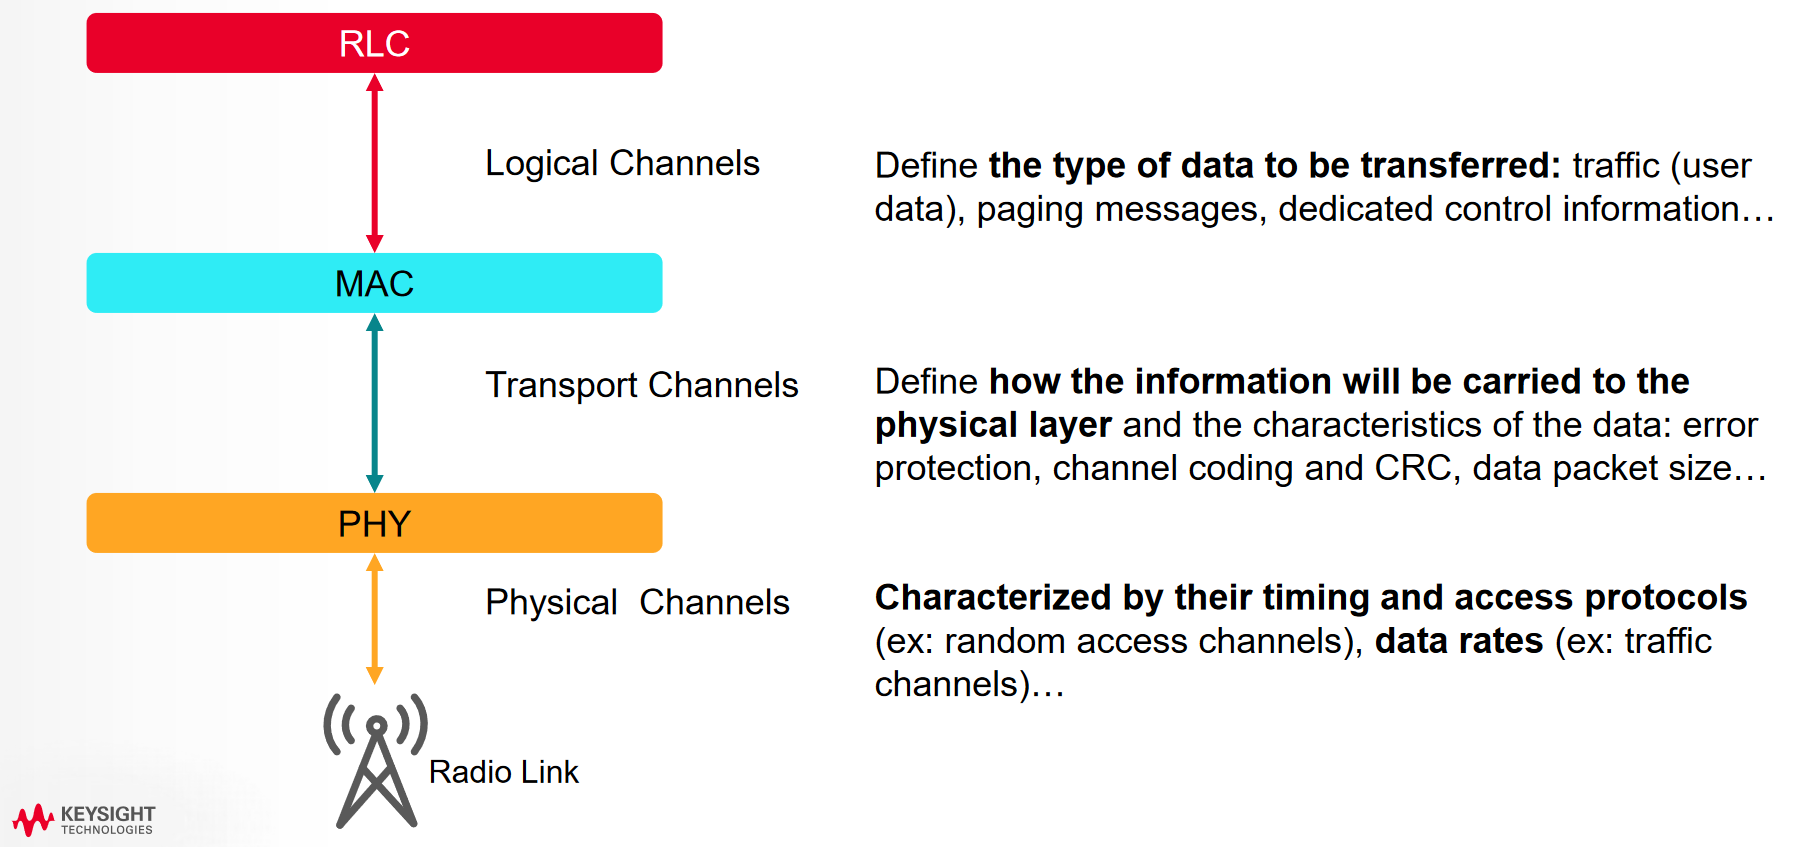
\includegraphics[width=0.9\textwidth]{res/nr-types-channels.png}
    \caption{Different types of channels used in 5G, courtesy of \href{https://www.keysight.com/}{ Keysight technologies}}
    \label{fig:nr-types-channels}
\end{figure}

\subsection{TDD operation}
The most complex problem to solve when dealing with propagation delay is certainly the \ac{TDD} mode of operation. In this scenario, each user can communicate only inside its assigned time slots.

Differently from 4G, where a predefined pattern was in place when allocating downlink and uplink allocations in a radio frame, in New Radio this is done much more flexibly using a plethora of parameters such as the periodicity of UL and DL transmissions, the number of consecutive DL and UL slots and symbols at the beginning of each pattern and more.

\paragraph{}The important key concept is that all the scheduler work has to account for the propagation delay. While in terrestrial communications guard periods of six symbols when switching from downlink communications to uplink communications is sufficient to account for the delay in a 32Km-radius cell, and timing advance commands can account for the different propagation delays experienced by users located in the center of the cell and users located in the cell edge \cite{gsma-5g-tdd-sync}, the same cannot be said for non-terrestrial use cases, where the distances that come into play are much longer, therefore any delay is orders of magnitude higher.

\section{Accounting for propagation delay in scheduling}

\subsection{Problem description}
\label{ss:propdelay-problem-desc}
\paragraph{}
The first encountered problem while implementing a non-terrestrial communication scenario in the simulator was the inability of the scheduler to account for the propagation delay when allocating radio resources to the connected user equipment on the ground.

The implementation of the 5G scheduler in ns-3 is designed to allocate resources less than a single subframe in advance, and since each subframe has a duration time of 1ms, the resource grant was already expired by the time it was able to reach the \ac{UE}, since it was referring to a past subframe.

\paragraph{Example} Consider a scenario with a propagation delay $\tau_p$ of 6ms. The \ac{UE} sends a request for uplink resources at time $t_0$ since it has some data to send. In the terrestrial scheduler implementation, the \ac{gNB} would receive such request at $t_0+\tau_p=6\textit{ms}$ and, provided that other transmissions have not been scheduled yet, grant the \ac{UE} the possibility to transmit in the following slot, which will start after 1ms at $t_0+\tau_p+t_{\textit{slot}}=7\textit{ms}$. However, this grant will reach the \ac{UE} only after another propagation delay, therefore at $t_0+2\tau_p=12\textit{ms}$, when it will already be too late.

\subsection{Proposed solution}
\label{ss:propdelay-problem-sol}
The implemented solution assumes that the scheduler has knowledge of the propagation delay. This is a reasonable assumption since systems such as GPS already rely on a precise estimation of the delay between the user on the ground and the satellite.

The scheduling then proceeds as normal with the only difference being that the information regarding the propagation delay is used to postpone the allocated symbols. 

\paragraph{Example} Consider the same scenario of the previous example in section \ref{ss:propdelay-problem-desc}. The new implementation of the scheduler accounts for the propagation delay by allocating the first available slot after $\tau_p$, so the time for the grant to reach the \ac{UE} is accounted for, and the \ac{gNB} marks the slot after $2\tau_p$ as reserved.

The last part of reserving a different slot is not as immediate. However, this mechanism needs to be in place because of the behavior depicted in Figure \ref{fig:scheduler-allocations-pd}, where a scenario with propagation delay of 5 slots (roughly 1,2ms) is considered:


\begin{itemize}
    \item \ac{UE} sends the scheduling request to \ac{gNB} at frame 1, subframe 0, slot 0.
    \item The \ac{SR} reaches the \ac{gNB} after $1\tau_p$ of 5 slots and the \ac{UE} is scheduled to transmit at frame 1, subframe 2, slot 2 since there is some noticeable propagation delay.
    \item The \ac{SR} reaches the \ac{UE} at frame 1, subframe 2, slot 2, and the \ac{UE} can transmit right away.
    \item The packet reaches the \ac{gNB} after another $\tau_p$, hence the base station needs to know that it cannot schedule other transmissions to take place in this slot, otherwise interference and collisions may arise.
\end{itemize}

\begin{figure}[ht]
    \centering
    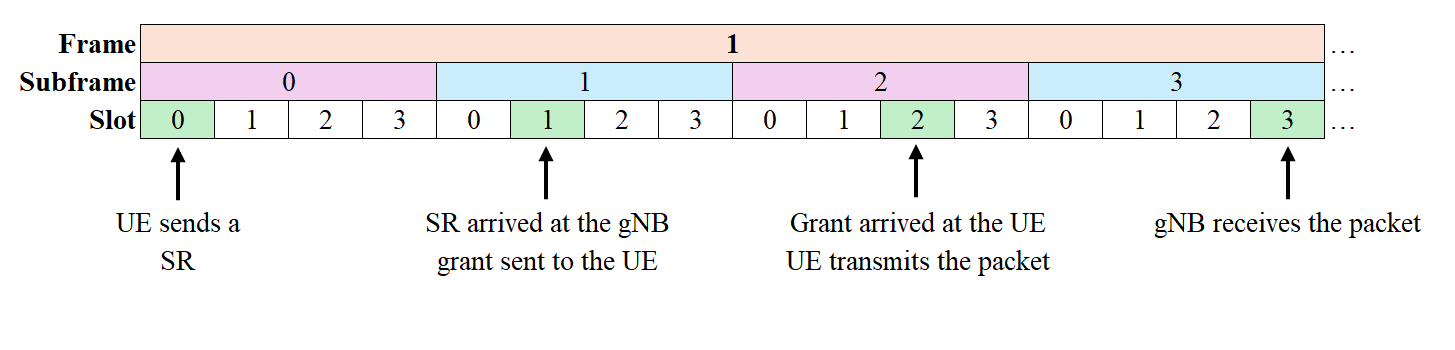
\includegraphics[width=0.9\textwidth]{res/scheduler-allocation-pd.png}
    \caption{Difference between allocated slot and gNB reception}
    \label{fig:scheduler-allocations-pd}
\end{figure}

\section{BSR timer}

After implementing the solution discussed in the previous point in the ns-3 network simulator, allowing the communication to take place, some other irregularities were found regarding the periodic buffer status report timer, as followingly described. 

\subsection{Problem description}

\paragraph{Reduced latency}

Figure \ref{fig:lat-saw} shows a rather peculiar trend regarding latency. The expectations were of a linear increase in latency with a slope of 3, where every packet arrived at the destination after three times the propagation delays. The reasoning behind this expectation was that every packet generated by the application should have triggered a scheduling request received by the \ac{gNB} after $1\tau_p$, a grant to be emitted requiring another $\tau_p$ to reach back to the \ac{UE}, and finally the transmission to be received by the \ac{gNB} after the third propagation delay.

The observed pattern did not match any of the expectations. The output plots obtained from the simulation campaign showed a nonlinear saw tooth behavior presenting values that consistently stayed under the expected $3\tau_p$ threshold value (Fig. \ref{fig:lat-saw}).

\begin{figure}[ht]
    \centering
    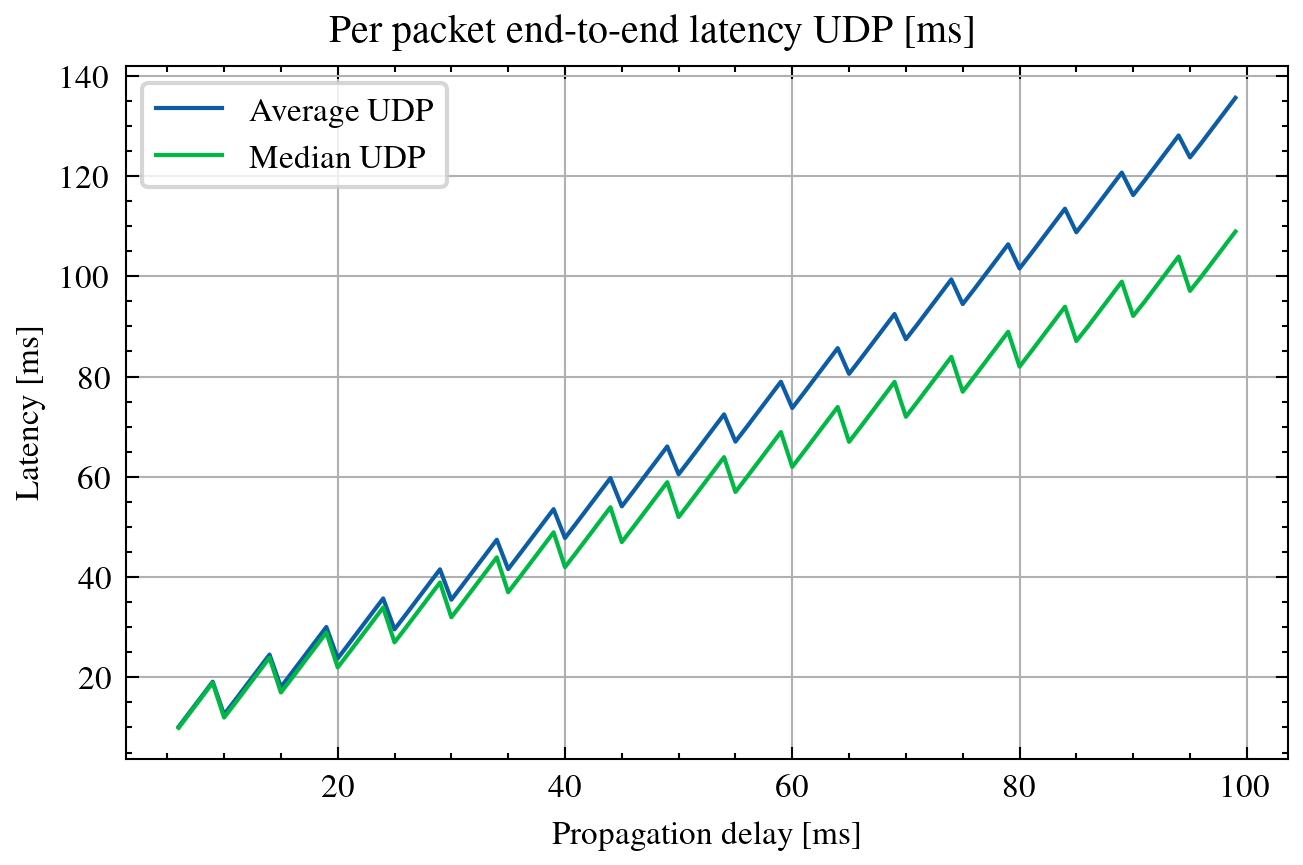
\includegraphics[width=0.9\textwidth]{res/lat-udp-saw.png}
    \caption{E2E latency vs. propagation delay with periodic \ac{BSR}}
    \label{fig:lat-saw}
\end{figure}

\paragraph{Periodic buffer status reports} Further investigation on the subject allowed to identify numerous buffer status reports sent from the \ac{UE} to the \ac{gNB} at regular intervals of 10ms, even when no new packets were produced by the application.

This behavior happens because the implementation of 5G \ac{MAC} layer includes a periodic \ac{BSR} that the \ac{UE} sends to the \ac{gNB} as long as the transmission buffer contains some pending data.
The details of this mechanism are documented in Section 5.4.5 of the standard \cite{etsi-mac-specification}, where it is also stated that the default interval between those periodic \ac{BSR} is of 10ms.

This characteristic was meant to act as a safeguard against lost scheduling requests, and does not account for the propagation delay at all. The \ac{UE} therefore continues to send additional buffer status reports at regular 10ms intervals even though the previous ones were not lost, but still travelling towards the base station.

\paragraph{}
Figure \ref{fig:diagram-wasted-capacity} can provide a visual clue to understand this behavior. The arrival of packet p1 at time zero triggers the transmission of a first \ac{SR}. Since this scenario has a propagation delay of 20ms, the \ac{SR} will arrive at the g-NodeB at time 20ms. However, the \ac{BSR} timer expires in 10ms by default, so during a single round-trip time the \ac{SR} is repeated four times. The green arrows marked with a capital G denote all the grants issued to the \ac{UE}. Only one of the four depicted will actually be used by the intended packet, effectively wasting three out of four transmission opportunities that could have been allocated to other users waiting to transmit.

\begin{figure}[ht]
    \centering
    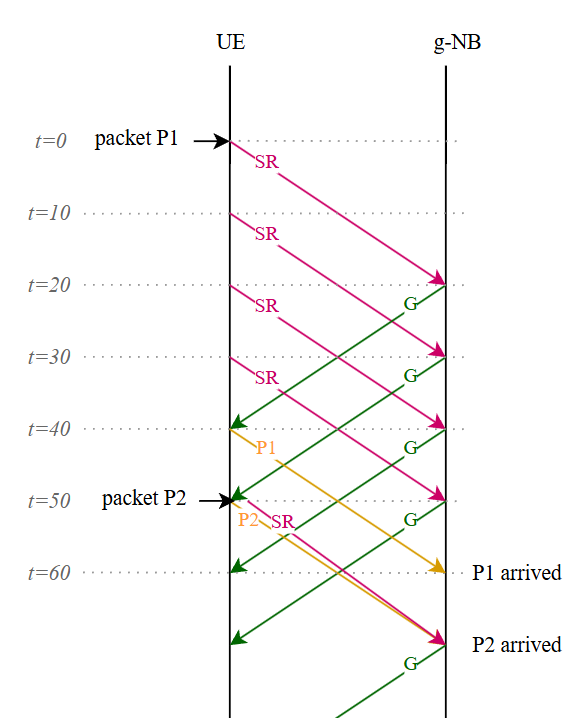
\includegraphics[width=0.8\textwidth]{res/diagram-wasted-grants.png}
    \caption{Packet diagram with periodic \ac{BSR}}
    \label{fig:diagram-wasted-capacity}
\end{figure}

The reduction in latency was observed because newly arrived packets could, in certain situations, make use of the resource grants that were meant for the previous packets but have yet to arrive at the \ac{UE}. Consider the arrival of the second packet (P2) in figure \ref{fig:diagram-wasted-capacity}. It triggers another \ac{SR}, but a grant is received immediately after, therefore allowing for an immediate transmission of the second packet, which will experience a latency of only a single propagation delay. This instantaneous grant is nothing but the result of the previous \ac{SR} storm originated from the \ac{UE} itself.

While this can present some beneficial aspects such as the reduced overall latency, it originates from a behavior that is outside the original design intentions. Moreover, this approach is particularly greedy, leading to wasted capacity.

\subsection{Proposed solution}

After the successful identification and characterization of the problem, the  solution consisted of the implementation of a simple adaptive algorithm that would dynamically set the \ac{BSR} timer to a value of twice the propagation delay plus a constant of 4ms that accounts for the processing times.

\paragraph{Area of potential improvement}
The implementation of the aforementioned solution, however, while working as intended, had the expected but unwelcomed effect of increasing the overall latency of the system, since all the additional grants required by previous packets and that newly generated ones could exploit were no longer available.

This unexpected problematic behavior of wasted transmission opportunities accidentally also unveiled the potential of preemptively transmitting additional scheduling requests, so that future packets could be sent with a lower latency.

If implemented correctly, the \ac{UE} could adopt a predictive approach towards its traffic needs for the near future depending on the type of application, and send the \ac{gNB} some scheduling requests for packets that have yet to be generated.

\section{Inflated BSR}

\subsection{Problem description}
Another problem occurred when the interval between the packets generated by the application, i.e. the packets interarrival times, was smaller than a single round-trip time. 

\paragraph{}
The arrival of each packet automatically triggers the transmission of a scheduling request by the \ac{UE}. However, each request is made for the whole transmission buffer. This causes a problem when many packets arrive before the \ac{gNB} has the chance to respond with the appropriate resource grant.

Referring to Figure \ref{fig:inflated-bsr-diag}, we can see that the arrival of the first packet in the transmission buffer of the \ac{UE} triggers the transmission of a \ac{SR} for a single packet. The second packet P2 arriving after 10ms triggers another request, however this second request is cumulatively made for the full buffer length, regardless of the fact that the first \ac{SR} is still pending. This is denoted by the writing "SRx2". Packets P3 and P4 behave in the same way, triggering requests for the allocation of three and four additional packets respectively.

Finally, the grants begin arriving at the \ac{UE}. The first 1-packet grant allows for the transmission of P1, while the second grant, requested for two packets, allows for the transmission of packets P2 and P3. The third grant, which corresponds to a previous request for 3 packets and could therefore allow the transmission of 3 packets, can now only be used by P4, wasting 2/3 of its potential capacity. 

The last grant, that would allow the \ac{UE} to transmit 4 consecutive packets, is completely wasted since the send buffer is found empty.

\begin{figure}[ht]
    \centering
    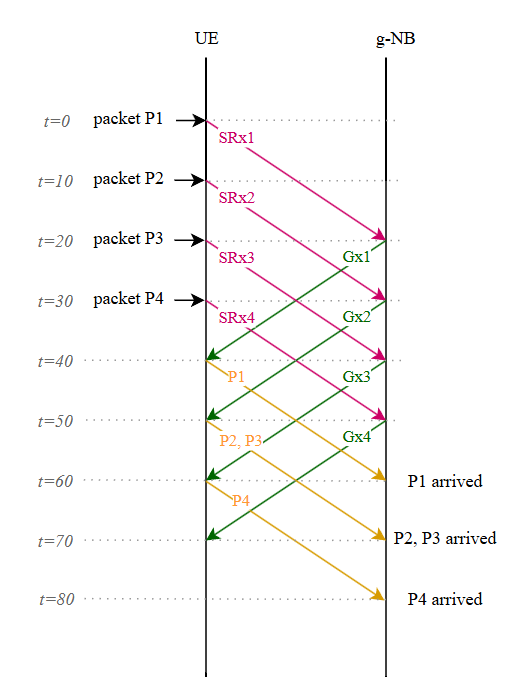
\includegraphics[width=0.8\textwidth]{res/diagram-inflated-bsr.png}
    \caption{Packet diagram for interarrival times smaller than propagation delay}
    \label{fig:inflated-bsr-diag}
\end{figure}

\paragraph{Repercussions}
The described behavior caused the physical throughput to be significantly higher than the set application source rate, and it rapidly increased with the propagation delay. Figure \ref{fig:phy-thr-runaway} shows the observed physical throughput for a source rate of 160Kb/s, indicating that a lot of radio resources are being wasted to transmit few data.

\begin{figure}[ht]
    \centering
    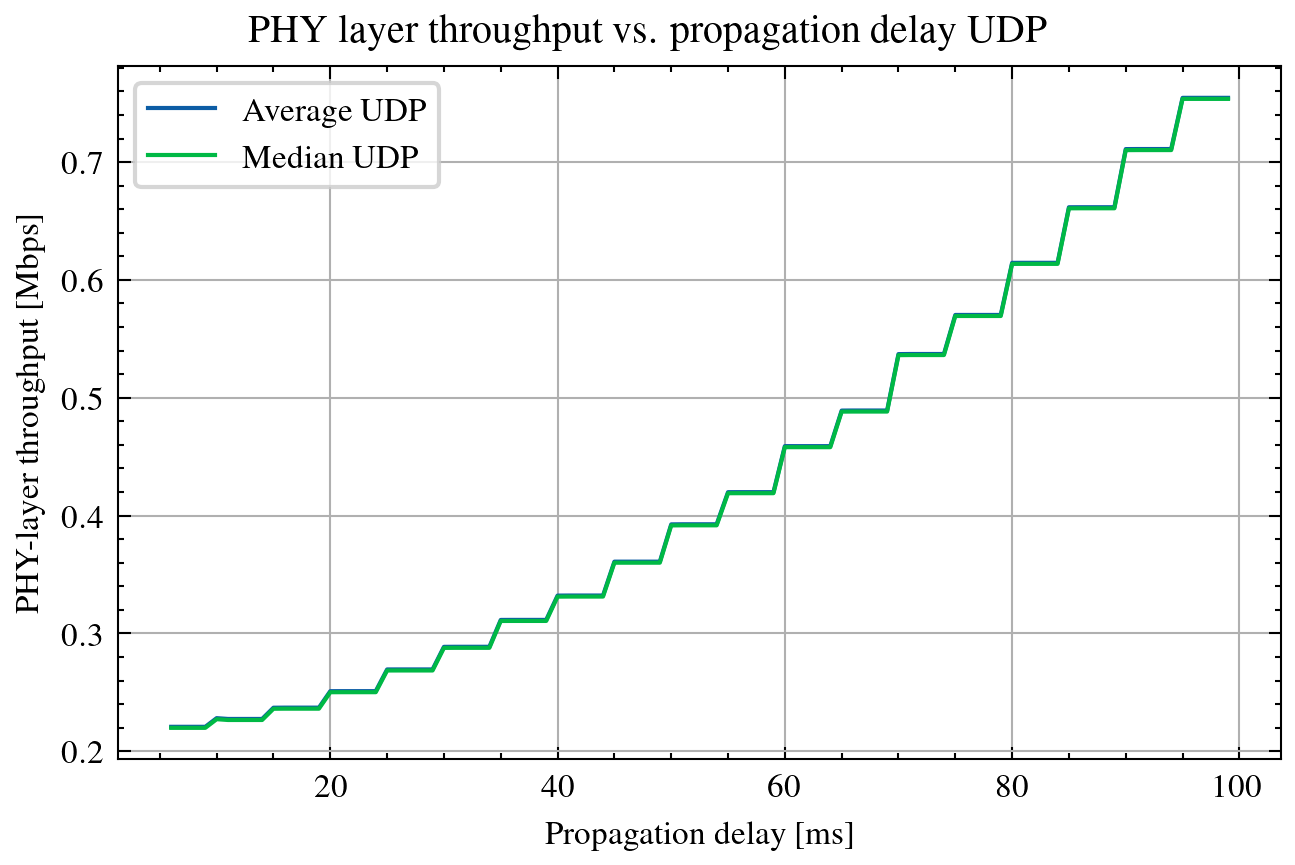
\includegraphics[width=0.9\textwidth]{res/phy-thr-udp-runaway.png}
    \caption{Physical throughput vs. propagation delay with periodic \ac{BSR}}
    \label{fig:phy-thr-runaway}
\end{figure}

\subsection{Proposed solution}

Various different approaches could be undertaken in order to tackle this problem. Nonetheless, a comprehensive study detailing upsides and downsides of each of them is outside the scope of this work. 

The implemented solution consists of a modification to the \ac{SR} algorithm that limits the requests to only account for the newly received data, therefore disabling the cumulative behavior. If a packet is already in the buffer when a new one arrives, the scheduling request only asks the size of the second packet to be allocated.

As mentioned before, the implementation of a smarter algorithm, capable of predicting the traffic needs of the \ac{UE} could be employed to reduce the latency. 

\section{Reordering timer}

\subsection{Problem description}
\paragraph{Fragmentation}
The packets interarrival times are not necessarily multiples of the propagation delay, and the resources that the g-NodeB grants to the \ac{UE} are usually a few bytes larger than the packet size. This happens because, even though 5G scheduling can be done on a much finer granularity than 4G scheduling, the base station still cannot grant values that are smaller than a single symbol, so the general rule is to allocate the minimum number of symbols whose cumulative size is greater or equal to the requested allowance.

This misalignment between packet size and transmission opportunities allows for packets to be split in smaller pieces. If two packets of 200B each are waiting in the buffer to be transmitted, and a resource grant for 220B arrives at the \ac{UE}, the first packet can be completely transmitted, but it would be wasteful not to use also the 20 additional bytes that were granted, so the second packet is split and only its first 20B are transmitted. The remaining 180B will wait for the next opportunity.

\paragraph{PDCP}
The detailed implementation of the \ac{PDCP} layer can be found in the \ac{3GPP} technical specification \cite{pdcp-spec-3gpp}, while the diagram describing its functionality has been reported in Figure \ref{fig:pdcp-functionalities}. This layer offers reordering services by employing a sequence number, integrity protection and ciphering if the packet in question is associated to a \ac{PDCP} \ac{SDU}, and duplication and routing when operating split bearers.

The observed problem, as the propagation delay increases, is related to an expiring timer when reassembling the packets at the \ac{PDCP} layer. The so-called reordering timer (t-reordering), which despite the name also affects the recomposition of fragmented packets, is not configured for the use in a non-terrestrial scenario, and it expired before the second half of the packet managed to arrive. 

This re-ordering functionality of \ac{PDCP} layer is in place to ensure a sequential delivery of packets to the upper layers. In case of missing packets, the behavior is to wait until either the packets arrive or the reordering timer expires \cite{efficient-reassembly-pdcp}. It was observed that this timer also started when the \ac{PDCP} layer was waiting for the arrival of the second part of a fragmented packet. However, due to the high propagation delay, the arrival of the second half was not possible before the timer expiration, leading to the packet being discarded.

Should the reordering timer be set too high, it may cause additional latency, and, if set too low, it might cause many packets to be discarded, as in the case that was simulated during this work \cite{efficient-reassembly-pdcp}.

\begin{figure}[ht]
    \centering
    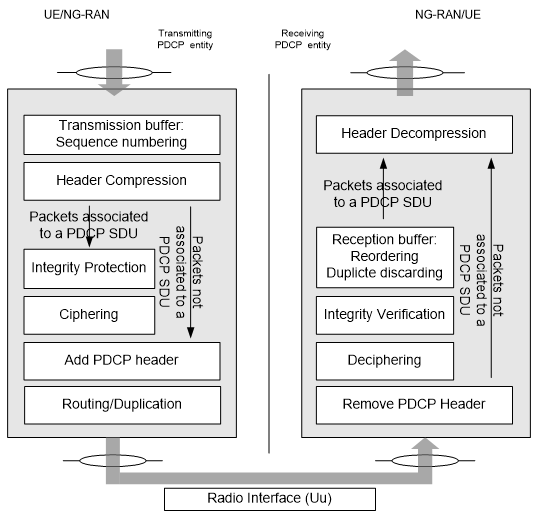
\includegraphics[width=0.9\textwidth]{res/pdcp-functionality.png}
    \caption{PDCP diagram \cite{pdcp-spec-3gpp}}
    \label{fig:pdcp-functionalities}
\end{figure}

\subsection{Proposed solution}
Since the problem is linked to the expiration of a timer, and the propagation delay of \ac{NTNs} is much larger than the terrestrial case, the implemented solution consisted in the increase of the default timer value to account for the additional delays.

Since the use of timers always bear trade-offs depending on their value, in this case either being a higher latency or a higher packet discard ratio, there can not be a one-fits-all approach: the differences in propagation delays between satellites orbiting at different altitudes are so drastic that the implementation of a single default value would lead to suboptimal performances in every possible scenario. A much better approach would be to dynamically adapt the reordering timer accounting for the estimated propagation delay, similarly as the proposed solution for the scheduling problems in Section \ref{ss:propdelay-problem-sol}.